\subsection{Vorticity and polarization}

An interesting open question for relativistic fluids is to what extend the spin degrees of freedom thermalize locally and to what extend spin polarization results as a consequence of the fluid motion. Intuitively, one might expect that spin aligns locally with the rotational motion of the fluid as measured by vorticity, corresponding to the curl of the fluid velocity.

The relativistic generalization of the non-relativistic fluid vorticity is non unambiguous, however. The vorticity of a fluid in local equilibrium is characterized by the so-called thermal vorticity tensor, corresponding to $\omega_{\mu\nu} = \frac{1}{2} (\nabla_\nu \beta_\mu - \nabla_\mu \beta_\nu)$ where $\beta_\mu=u_\mu / T$ is the ratio of fluid velocity to temerature \cite{Becattini:2013fla}. This thermal vorticity has then contributions from rotational motion, local fluid acceleration, and temperature gradients. It has been argued, that local spin polarization should follow this thermal vorticity. If this holds at chemical freeze-out, one should be able to find traces of the thermal vorticity in the polarization of particles and resonances with spin, such as Lambda and (anti-) Lambda resonances.

Spin polarization is in this picture closely tied to angular momentum of the expanding fireball. For non-central events, an angular momentum of the produced matter can result that points into the transverse plane, orthogonal to the event plane. Via the spin-vorticity coupling mechanism, this leads to global polarization in the transverse plane (along global angular momentum) which has recently also been found experimentally at RHIC [citations]. For this global effect following global angular momentum, one expects a decreasing magnitude with increasing collision energy and the effect is expected to be relatively small at LHC energies. 

In addition to that, there is also the expectation of a azimuthally dependent, longitudinal polarization (in the direction of the beam pipe). This is mainly a consequence of an azimuthal dependence of local acceleration and temperature gradient and should lead for non-central collisions mainly to an elliptic modulation of spin polarization. This effect has a weaker dependence on collision energy and should be almost as large at the LHC as at RHIC \cite{Karpenko:2017dui}. It would be highly interesting to investigate polarization effects of Lambdas and other resonances in more detail at the LHC and to map out the dependence on azimuthal angle, rapidity, transverse momentum etc.




\begin{itemize}
	\item
The estimation for the LHC energy $\sqrt{s_{NN}}=2.76$ TeV indicate the strength of Abelian magnetic field is $eB \sim 1.0$ GeV$^{2}$ very shortly after collisions and it decreases down to the $eB \sim 200$ MeV$^{2}$ for time $\tau \sim 0.1$ fm/$c$ without taken into account the electroconductivity of the quark-gluon matter \cite{AHEP-2014-193039-2014,JPCS-668-012129-2016,JPCS-675-022021-2016}. Therefore one can expect $|\Delta P|=0.61eB/m_{p}T \sim (4.3 \pm 0.7) \times 10^{-4}$ for the temperature of the quark-gluon plasma $T=(304 \pm 51)$ MeV \cite{NPA-904-905-573c-2013}. Here $m_{p}$ is the proton mass, $\Delta P \equiv P_{\Lambda}-P_{\bar{\Lambda}}$ is the difference in polarization of primary $\Lambda$ and $\bar{\Lambda}$ \cite{PRC-95-054902-2017}. This estimation for $|\Delta P|$ is some smaller than that at RHIC energies due to hotter medium at the LHC. But it should be noted the electroconductivity will lead to noticeably weaker time dependence of the $eB$ \cite{AHEP-2013-490495-2013} and the conductivity may compensate the growth of $T$ and provides the increase of the $|\Delta P|$. Moreover the pass from RHIC to the LHC energy leads to the significant growth of the peak value for $eB$. Thus for HE--LHC the magnitude of $\Delta P$ is expected similar or even larger than at RHIC energies. Furthermore the higher energy of the HE--LHC project provides the novel opportunity for study of polarization of heavier hyperons (for instance, $\Sigma$) in hot environment.
\end{itemize}

\begin{figure}[!htb]
\begin{center}
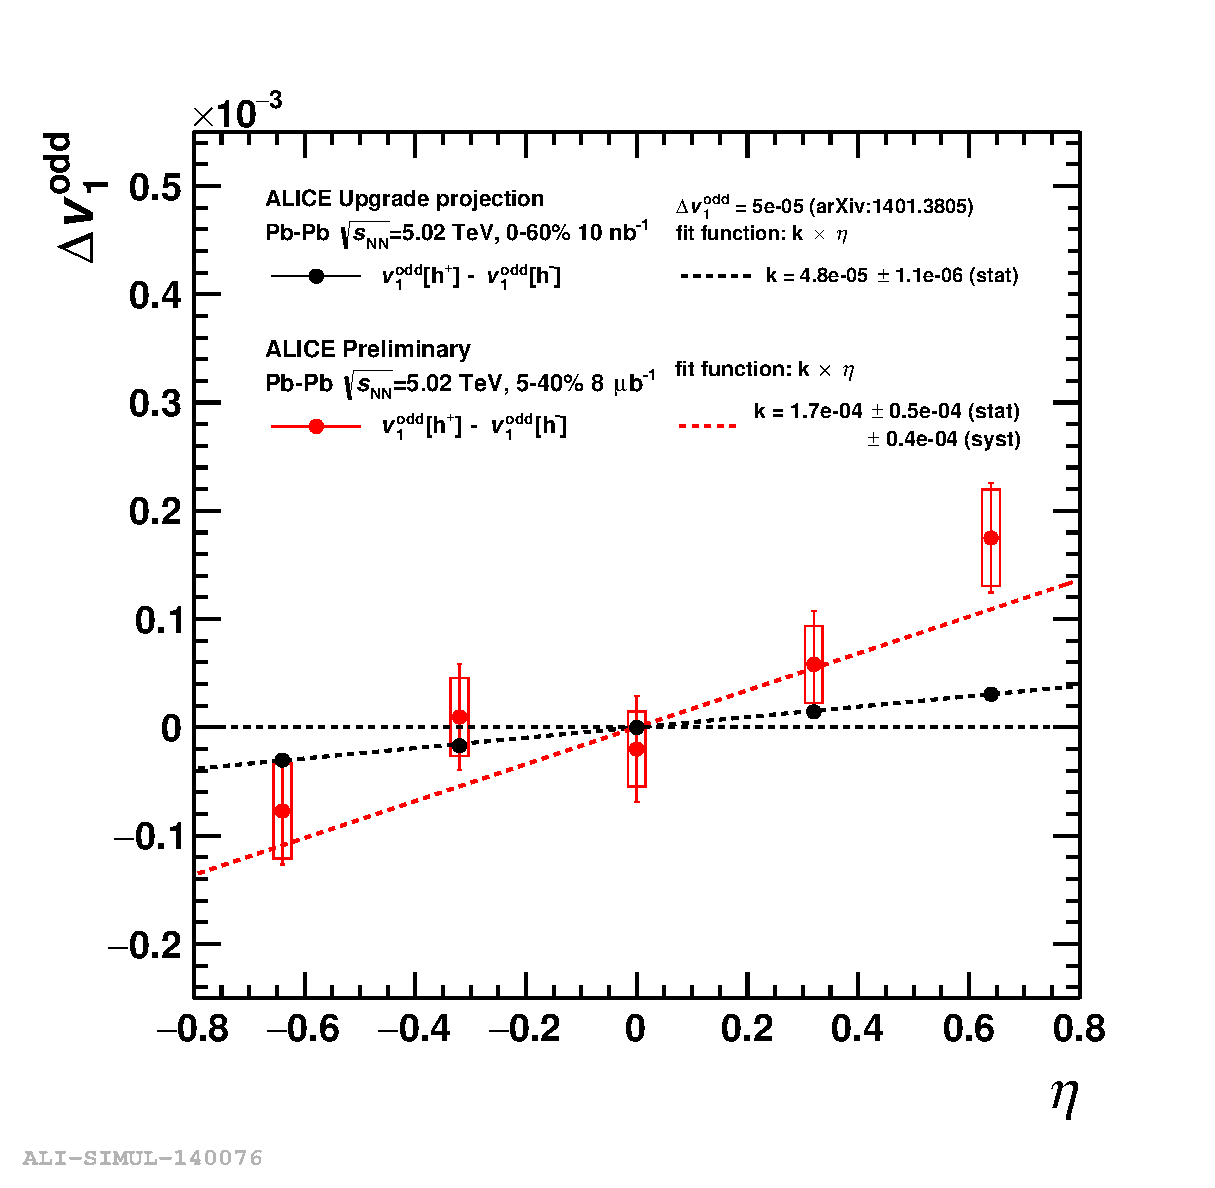
\includegraphics[width=0.8\textwidth]{\main/flow/figs/alice_projection_deltav1ch_stat8}
\caption{
}
\label{fig:alice_delta_v1}
\end{center}
\end{figure}


\begin{figure*}[!htb]
\begin{center}
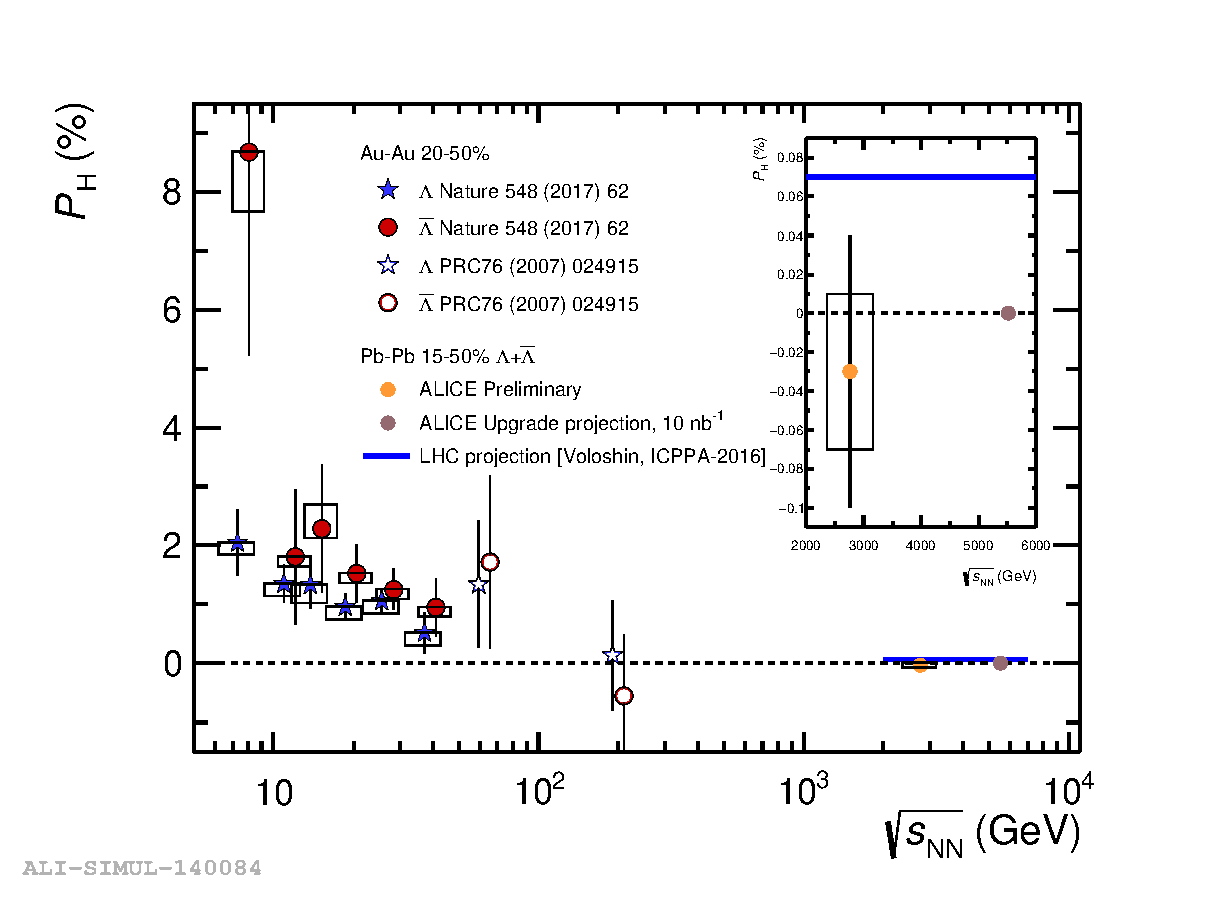
\includegraphics[width=0.8\textwidth]{\main/flow/figs/alice_projection_lambda}
\caption{Global polarization of $\Lambda$ and $\bar{\Lambda}$ as a function of the collision energy $\sqrt{s_{NN}}$ for semi-central heavy ion collisions. Open boxes
and vertical lines show systematic and statistical uncertainties,
respectively. Main panel: the data points for $\bar{\Lambda}$ are slightly horizontally shifted for visibility. Inner panel: the LHC energy domain is shown more detailed.
}
\label{fig:alice_lambda}
\end{center}
\end{figure*}

Fig. \ref{fig:alice_lambda} presents the energy dependence of the global polarization of $\Lambda$ and $\bar{\Lambda}$ for the semi-central heavy ion collisions. The RHIC results show the decrease of polarization at higher $\sqrt{s_{NN}}$. But $\Lambda$ and $\bar{\Lambda}$ demonstrate the finite global polarizations even at highest RHIC energy $\sqrt{s_{NN}}=200$ GeV \cite{PRC-98-014910-2018}. The preliminary ALICE data point at $\sqrt{s_{NN}}=2.76$ TeV is close in magnitude with results at $\sqrt{s_{NN}}=200$ GeV. But the ALICE upgrade projection at twice large collision energy corresponds to the zero polarization with very high precision. Therefore the study of global polarization of $\Lambda$ and $\bar{\Lambda}$ within HL--LHC project allows the unambiguous conclusion with regard of the values of this physics quantity in TeV-energy domain.    
